\documentclass[a4paper, 12pt]{article}
\usepackage[utf8]{inputenc}
\usepackage[english]{babel}
\usepackage{csquotes}

%   Fixa n / log n plot
%   Bestäm alla algoritmer
%   Förklara mersene / fermat primes
%   Fixa algoritmer samt kod (driver)
%   Köra tester
%   bara fortsätt
%   Titta så att robbin har inkluderat källor
%   Fixa formatering samt stavning

%---Ploting---------------------------------------------
\usepackage{pgfplots}
\pgfplotsset{compat=1.16}
%-------------------------------------------------------

%---Writing symbols-------------------------------------
\usepackage{amsfonts}
\usepackage{enumerate}
%-------------------------------------------------------

%---Boxes-----------------------------------------------
\usepackage[framemethod=tikz]{mdframed}
%-------------------------------------------------------

%---Python----------------------------------------------
\usepackage{pythonhighlight}
%-------------------------------------------------------

%---Pictures--------------------------------------------
\usepackage{fancyhdr} % Good frontpage
\setlength{\headheight}{89pt}

\usepackage{graphicx} % Managing pictures
\graphicspath{ {./images/} }
%-------------------------------------------------------

%---References------------------------------------------
\usepackage[sorting=none]{biblatex}
\addbibresource{references.bib}
%-------------------------------------------------------

%---Makes Table of Contents clickable-------------------
\usepackage{url}
\usepackage{hyperref}
\urlstyle{same}
\hypersetup{
    colorlinks=true,
    linktoc=all,
    linkcolor=black,
    urlcolor=cyan,
}
%-------------------------------------------------------

%---Subfiles--------------------------------------------
\usepackage{subfiles}
%-------------------------------------------------------

\title{Understanding How the Largest Primes Came to Be}
\author{Ibrahim Abdulhussein, \\ Robin Brusbo}
\date{April 20, 2020}

\begin{document}

\makeatletter

\begin{titlepage}
    \thispagestyle{fancy}
    \renewcommand{\headrulewidth}{0pt}
    \renewcommand{\footrulewidth}{0pt}
    \lhead{
\includegraphics[scale=0.4]{logo.jpg}}
    \cfoot{}
    \hbox{}\vfill
    \begin{center}
        {\LARGE\@title}\\[2em]
        {\large\@author}\\[1em]
        {\large\@date}\\[6em]
        \fbox{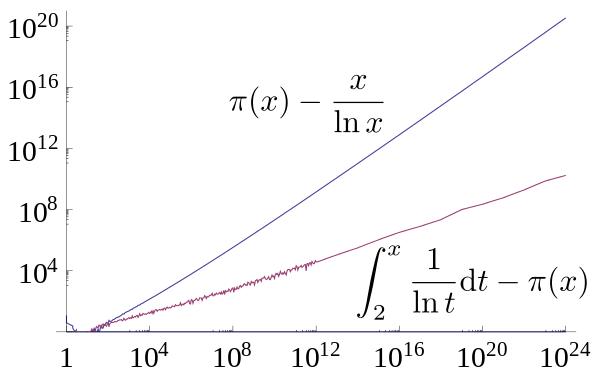
\includegraphics[scale=0.6]{frontpage.png}}\\
        \footnote{The Prime Number Theorem \cite{theorem:prime_num}}
    \end{center}
    \vspace{3cm}\vfill
\end{titlepage}

\makeatother

\newpage
%------------------------------------------------------
\section*{Abstract}

\subfile{abstract.tex}

\newpage
%-------------------------------------------------------
\tableofcontents

\newpage
%-------------------------------------------------------
\section{Introduction}

\subfile{introduction.tex}

\newpage
%-------------------------------------------------------
\section{Definitions}

\subfile{definitions.tex}

\newpage
%-------------------------------------------------------
\section{Materials and Methods}

\subfile{materials_methods.tex}

\newpage
%-------------------------------------------------------
\section{Results}

\subfile{results.tex}

\newpage
%-------------------------------------------------------
\section{Discussion}

\subfile{discussion.tex}

\newpage
%-------------------------------------------------------
\section{Conclusion}

\subfile{conclusion.tex}

\newpage
%-------------------------------------------------------
\section{Acknowledgments}

\subfile{acknowledgments.tex}

\newpage
%-------------------------------------------------------
\section{References}

\emergencystretch=0.25em
\printbibliography[heading=none]

\newpage
%-------------------------------------------------------

\end{document}